\documentclass[11pt]{article}
\usepackage{amsmath, amsfonts, amsthm, amssymb}  % some math symbols
\usepackage{lmodern}  % a modern version of latex's famous default font. 
\usepackage{microtype}
\usepackage{fullpage}
\usepackage[x11names, rgb]{xcolor}
\usepackage{graphicx}
\graphicspath{ {./figures/} }
\usepackage{tikz}
\usepackage{mathtools}
\usetikzlibrary{automata, positioning, decorations,arrows,shapes}
\providecommand\given{}
\usepackage{etoolbox}
\usepackage{enumerate}
\usepackage{listings}
\usepackage{dsfont}

\setlength{\parindent}{20pt}
\setlength{\parskip}{5pt plus 1pt}

\newtheorem{theorem}{Theorem}[section]
\newtheorem{corollary}{Corollary}[theorem]
\newtheorem{lemma}[theorem]{Lemma}

\providecommand\given{}
\DeclarePairedDelimiterXPP\prob[1]
{\mathbb{P}}()
{}{
\renewcommand\given{\nonscript\:\delimsize\vert\nonscript\:\mathopen{}}
#1}
\DeclareMathOperator*{\argmax}{arg\,max}
\DeclareMathOperator*{\argmin}{arg\,min}
\makeatletter
\renewcommand*\env@matrix[1][*\c@MaxMatrixCols c]{%
  \hskip -\arraycolsep
  \let\@ifnextchar\new@ifnextchar
  \array{#1}}
\makeatother

\providecommand\expec[1]
{\mathbb{E}[#1]}


\def\indented#1{\list{}{}\item[]}
\let\indented=\endlist

%%%%%%%%%%%%%%%%%%% Document Options %%%%%%%%%%%%%%%%%%%%%%
%%%%%%%%%%%%%%%%%%%%%%%%%%%%%%%%%%%%%%%%%%%%%%%%%%%%%%%%%%%

\begin{document}
On June 4, 1996, after years of hard work and \$370 million dollars in the
  making, the Ariane 5 rocket was ready for takeoff.
30 seconds after launch, the rocket veered off-course, triggering the
  self-destruct sequence and destroying the rocket.
The culprit---a software bug caused by an issue with the on-board computer’s
  number system.

Aren’t computers supposed to be good with numbers? 
Most computations in math and science are done in terms of the real numbers.
This includes numbers that are incredibly large and irrational numbers with
infinite digits after the decimal point.
Because computers only have a finite amount of space and computational power,
computers have to make tradeoffs between the range, precision, and computational
efficiency of the numbers represented in the computer system.

Most computers calculate using floating-point numbers.
Floating-point numbers are made up of three parts—the sign, which represents
  whether the number is positive or negative; a mantissa, which represents the
  significant digits of the number; and an exponent, which represent the number
  of places you have to move the decimal point.

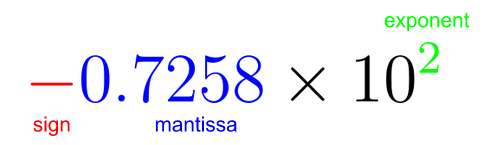
\includegraphics{floatingpointexample}

For example, take the number -72.58.
The number is negative, so the sign is negative.
The significant part, the mantissa, is 0.7258.
To get from 0.7258 to 72.58, you would have to move the decimal twice to the
  right, so the exponent is 2.
In a real computer, the sign, mantissa, and exponent would all be represented as some 
  number of bits (1s and 0s) in binary.
The exponent determines the range of numbers that can be represented and the
  mantissa determines the precision of numbers that can be represented.

The number of bits used to represent a number depends on the number format.
The baseline for number formats is the IEEE754 standard, which specifies a 
  half-precision format (16 bits per number), a single-precision format (32 bits per number),
  and a double-precision format (64 bits per number).
Although these are by far the most popular number formats and are used by most 
  modern computers, some special applications use different number formats 
  with different sizes of mantissa and exponent to fit their own
  priorities.
For example, bfloat16, a specialized number format developed at Google Brain for
  machine learning applications.
Like the IEEE754 half-precision format, bfloat16 uses 16 bits to represent
  each number, but because machine learning algorithms require a larger range
  of numbers while caring less about precision, bfloat16 has a smaller mantissa
  and a bigger exponent.

Although floating-point numbers are incredibly versatile, they have their
  limitations.
Floating-point errors can be difficult to identify and can lead to catastrophic
  amounts of error.
The goal of floating-point arithmetic is to produce the result that is as close
  as possible to the arithmetic done in the real numbers.
We say an expression error is the difference between the evaluated value of the
  expression and the closest floating-point number of that expression evaluated
  in the real numbers.


A common floating-point error is \textbf{cancellation}; when subtracting two numbers that are very
  close together, the result can be rounded to zero.
Suppose we want to know $(1 - 0.6) \times 10$, but our calculator always rounds to 
  the nearest whole number after every operation.
$(1 - 0.6)$ would be rounded to zero, and then $0 \times 0 = 0$, so the whole
  expression would compute to $0$.
What if, instead we had the expression $1 \times 10 - 0.6 \times 10$?
This expression should be equivalent to the first one, but let's look at how it computes.
$1 \times 10$ would round to $10$.
$0.6 \times 10$ would round to $6$.
Finally, $10 - 6 = 4$.
Oh no!
Even though these two expressions are supposed to be the same, rounding can make their
  results different!
The first expression evaluates to $0$ but the best approximation (the second expression) evaluates $4$.
Thus, we say that the \textbf{absolute error} is $4$.
This is a common error in floating-point arithmetic stemming from the way
  floating-point numbers are rounded.

Another common floating-point error is \textbf{overflow}.
Every floating-point number format has a maximum number that can be represented.
When an operation results in a number that is more than the maximum number, the result
  is rounded to the maximum number.
Suppose we want to know $\frac{8 + 8}{2}$, but our calculator has a maximum number of $10$.
$8 + 8 = 16$, which is more than $10$, so it would be rounded to $10$.
Finally, $\frac{10}{2} = 5$ (notice, we would get $5$ if we replaced $8$ with any integer larger than $4$).
What if, instead we had the expression $\frac{8}{2} + \frac{8}{2}$?
As before, this expression should be equivalent to the first one, but let's look at how it computes.
$\frac{8}{2} = 4$.
$4 + 4 = 8$ 
Though these two expressions are supposed to be the same, overflow can make their
  results different!
The expression $\frac{8 + 8}{2}$ has an absolute error of $4$, since the expression evaluates to $4$ 
  but the best approximation $\frac{8}{2} + \frac{8}{2}$ evaluates to $8$.
This is another common error in floating-point arithmetic stemming from the finite nature of
  floating-point numbers.

As we saw in the previous examples, small changes to an expression can result
  in very different results!
Thankfully, we can improve floating-point expressions by doing simple rewrites.
In the example above, rewriting $(1 - 0.6) \times 10$ to 
  $1 \times 10 - 0.6 \times 10$ improves the accuracy of
  the expression by getting rid of the cancellation in $(1 - 0.6)$.

In more complicated expressions, errors may be more subtle and difficult to spot
  and rewriting an expression optimally can be a difficult task.
Often, mistakes in floating-point expressions takes an expert to spot
  and rewrite.
Thankfully, there are tools that can help in this process.

Herbie is a tool that is able to automatically rewrite floating-point
  expressions to improve accuracy.
It does this by applying algebraic rewrites repeatedly to an expression to create
  alternative expressions and chooses the most accurate expression.
However, Herbie is not perfect.
Herbie's automatically optimized expressions often aren't as accurate
  or concise as an expression hand-optimized by an expert.
Furthermore, in order to explore a wide range of rewritten expressions efficiently, 
  Herbie's rewrite rules are unfortunately mathematically imperfect.
For example, Herbie might rewrite $1$ to $\frac{x}{x}$, not accounting
  for the fact that when $x = 0$, there would be a divide-by-zero error.

There are also tools developed to identify and quantify floating-point errors.
NASA develops one such tool called PRECiSA.
Given a floating-point expression, PRECiSA will compute the maximum absolute error of 
  the given expression and generate computer 
  code annotated with warnings about the computed error.
NASA uses PRECiSA in safety-critical applications such as rockets and unmanned drones,
  which require absolute certainty in their calculations;
  to ensure correctness, all of PRECiSA's results are mathematically provable.
However, unlike Herbie, PRECiSA doesn't do any expression rewriting.
If the input floating-point expression is inaccurate, the generated computer code will still be
  inaccurate, albeit with proof of its inaccuracy.

One idea is to use Herbie to optimize an expression before passing it to PRECiSA.
This way, the generated computer code will be more accurate, while still benefitting from
  the mathematical guarantees generated by PRECiSA.
Unfortunately, there are some complications.
Confidence in the results generated by this process requires proof that Herbie's optimized
  expression is mathematically equivalent to the original expression.
However, due to the imperfections in Herbie's rewrite rules, this is often not directly
  possible.
One workaround is to have a conditional proof instead; proving that an optimization is
  equivalent to the original when some condition holds.

\end{document}

